\documentclass[12pt]{article}
\usepackage[margin=3.0cm]{geometry}
\usepackage[french, english]{babel}
\usepackage[utf8]{inputenc}
\usepackage{graphicx}
\usepackage[hidelinks]{hyperref}
\usepackage{amsmath}
\usepackage{setspace}
\graphicspath{{Images/}
\geometry{legalpaper}}

\begin{document}
\begin{titlepage} 
	\large
	{
		\begin{center}
			UNIVERSITÉ DE SHERBROOKE\\Faculté de génie\\
			Département de génie électrique et génie informatique\\
			\vspace{3cm}
			{\LARGE\textbf{Principes de dynamique et méthodes numériques}}\\
			\vspace{2cm}
			\LARGE{Rapport APP2}\\
			\vspace{2cm}
			Présenté à\\l'équipe professorale de la session S4\\
			\vspace{2cm}
			Produit par\\Axel Bosco, Jacob Fontaine, Philippe Spino\\
			\vspace{1cm}
			\vfill{23 mai 2017 - Sherbrooke}
		\end{center}
	}
\end{titlepage}
\tableofcontents
\newpage
%\onehalfspacing
\section{Introduction}
Principes de dynamique et méthodes numériques
Dans le cadre du cour \textit{Principes de dynamique et méthodes numériques}, le mandat remit à la présente équipe était de rendre l'initiation des étudiants de la faculté de génie plus passionnante a l'aide d'un parcours à obstacles de style \textit{Wipe-out}.

\section{Design de la glissade}
Le devis émit par le WOQ demandais de calculer la trajectoire d'un glissade passant absolument pas des points cartésiens précis. Comme le montre la tableau 1, la glissade doit passer par tout les points.

\begin{center}
	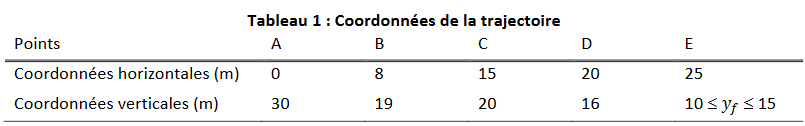
\includegraphics[scale=0.8]{tableau1}
\end{center}
Les valeurs de ce tableau sont les points de référence pour le approximation de la courbe de la glissade.

\subsection{Calculs}

\section{Design du débit d'eau}
\subsection{Calculs}

\section{Design du Ballon-mousse}
\subsection{Ballon Attrapé}
Dans cette situation, on présume que le participant attrape le ballon-mousse. Donc, on peut assumer alors qu'il y a une fusion du ballon-mousse et le participant après l'impacte en ceux-ci? Donc cela se résume à l'équation suivante:
\begin{equation}
m_p*v_p + m_b*v_b = (m_p + m_b)*v_{pb}
\end{equation}
En isolant $v_{pb}$, on obtien un valeur de :
\begin{equation}
v_{pb} = 5,59m/s
\end{equation}
À l'aide de cette vitesse, on doit règler la minutrie en sorte à ce que le participant ait quitté la plateform au complet avant que celle-ci s'ouvre.
\begin{equation}
\delta t_m = \frac{l_{trappe}}{v_{pb}}
\end{equation}
\begin{equation}
\delta t_m = \frac{3m}{5,59m/s} \approx{0,54}
\end{equation}
Et selon les standard imposés, la minutrie devait avoir une marge de manoeuvre de $0,02s$.
\begin{equation}
\delta t_m \approx{0,54 - 0,02} = 0,52sec
\end{equation}
\subsection{Ballon non attrapé}
Dans cette situation, le participant entre en collision avec le ballon sans l'attrapé. La collision entre le ballon-mousse et le participant à ce moment là est une collision plastique. Selon les requis du devis de WOQ, nous considérons le coefficient de récupération de $0,8$. Les valeurs de $V_{p_n}$ = 6.25$m/s$ et $V_{b_n}$ = -1.0$m/s$
\begin{equation}
e <= 0,8 = \frac{V'_{b_n} - V'_{p_n}}{V_{p_n} - V_{b_n}}
\end{equation}
suite a des manipulations algébrique, le résultat est:
\begin{equation}
{V_{b_n} - V_{p_n}} = 5,8
\end{equation}
\begin{equation}
V_b' = 5,8 + V_p'
\end{equation}
Il y a aussi l'équation suivante:
\begin{equation}
m_p.V_p + m_b.V_b = m_p.V_p' + m_b.V_b'
\end{equation}
\noindent
en substituant l'équation trouvé précédement, on obtien:
\begin{equation}
V_p' = \frac{m_p.V_p + m_b.V_b}{(m_b + m_p).V_b'}
\end{equation}
\begin{equation}
V_p' = 5.06m/s
\end{equation}
Donc, le temps requis pour traverser complètement la trappe est:
\begin{equation}
t_m = \frac{l_{trappe}}{V_p'} = 0,59 sec
\end{equation}

\section{Design de la minuterie}
Le devis avait un requis d'une marge de maneuvre de $0,02sec$ pour assurer la sécurité des participants concernant la trappe. Lorsque le ballon est attrapé, les temps est de $0,52sec$ et lorsque le ballon rebondit, le temps est de $0,59sec$.
\subsection{Calculs}
\begin{equation}
t_{m_f} < \Delta T_m - 0,02
\end{equation}
\begin{center}
et
\end{center}
\begin{equation}
t_{m_r} > \Delta T_m + 0,02
\end{equation}

Suite aux manipulations algébriques, le résultat est que 
\begin{equation}
\Delta T_m \approx 0,056 sec
\end{equation}

\section{Design du Coussin-Tampoline}
\subsection{Calculs}

\section{Design du Bassin}
\subsection{Calculs}

\section{Conclusion}


\end{document}